\subsection{External Configuration  (\textit{MK})}
Many configurations of aircraft were considered during initial design phase. First, a trade study was performed over similar aircraft that are either currently in service or have flown in the past. Table \ref{tabmk1} describes seven aircraft and some of their prominent external configuration characteristics. 

\begin{table}[H]
    \centering
    \caption{Quantitative Trade Study of Similar Aircraft}
    \begin{tabular}{|m{3cm}||c|c|c|c|c|}
    \toprule
    \label{tabmk1}
    \textbf{Aircraft} & \textbf{Tail Type} & \textbf{Wing Type} & \textbf{\# of Engines} & \textbf{2-class Seating} & \textbf{\# of Decks} \\
    \hline\hline
    Boeing 777-200 & Conventional & Low & 2 & 375 & Single \\
    \hline
    Airbus 340-600 & Conventional & Low & 4 & 440 & Single \\
    \hline
    Boeing 787-10 & Conventional & Low & 2 & 330 & Single \\
    \hline
    McDonnell Douglas MD-11 & Conventional (w/ engine) & Low & 3 & 323 & Single \\
    \hline
    Lockheed 1011-100 & Conventional (w/ engine) & Low & 3 & 304 & Single \\
    \hline
    Boeing 747-400 & Conventional & Low & 4 & 496 & Double \\
    \hline
    Airbus 350-900 & Conventional & Low & 2 & 315 & Single \\
    \bottomrule
    \end{tabular}
\end{table}
\clearpage
From the trade study, all seven of described aircraft featured a low-level wing along with a conventional tail. This is most likely due to the low-level wing providing space for a retractable landing gear along with simplicity of design. Thus, the team decided to go with a low-level wing.

The next external configuration decision was between a T-tail and a conventional tail. While the T-tail does reduce the risk of the tail stalling, it is much more difficult to design as the vertical tail has to support the entire weight of the horizontal tail. Alternatively, conventional tails are lighter and provide more simplicity in terms of design. Another benefit with conventional tails is that it offers more space to store fuel for the aircraft. Additionally, the team had already decided to utilize wing mounted engines, negating aerodynamic benefits causing the usage of T-tails on smaller regional and commercial aircraft with tail-mounted engines.  As shown from the trade study, conventional tails are very widely used in similar configuration commercial aircraft in today's market; thus the team decided to use a conventional tail configuration as illustrated in Figure \ref{fig3view}. 

Next, the number of engines on our aircraft along with the number of decks on the aircraft remained to be decided. The team decided to go with a single-level to provide simplicity in design as well reduced cost in manufacturing. Furthermore, two engines were chosen for our aircraft, mainly for the reduced maintenance cost corresponding to fewer engines as well as a smaller fuel cost. The proven reliability of modern engines in trans-oceanic flights also played a role in deciding to have two engines. Finally, the landing gear of our aircraft was determined to be a retractable, tricycle configuration further discussed in Section \ref{section: Landing Gear}. Figure \ref{fig3view} shows a top, left, front, and isometric view of the OpenVSP model of the aircraft. The Sam Mark 1 has a total length of 202 ft and a wingspan of 212 ft. The coordinate system for the aircraft starts at the tip of the nose cone of the aircraft, with the x-direction pointing out of the coordinate system, y-direction in the direction of the right wing, and z-direction down. 

\begin{figure}[H]
        \centering
        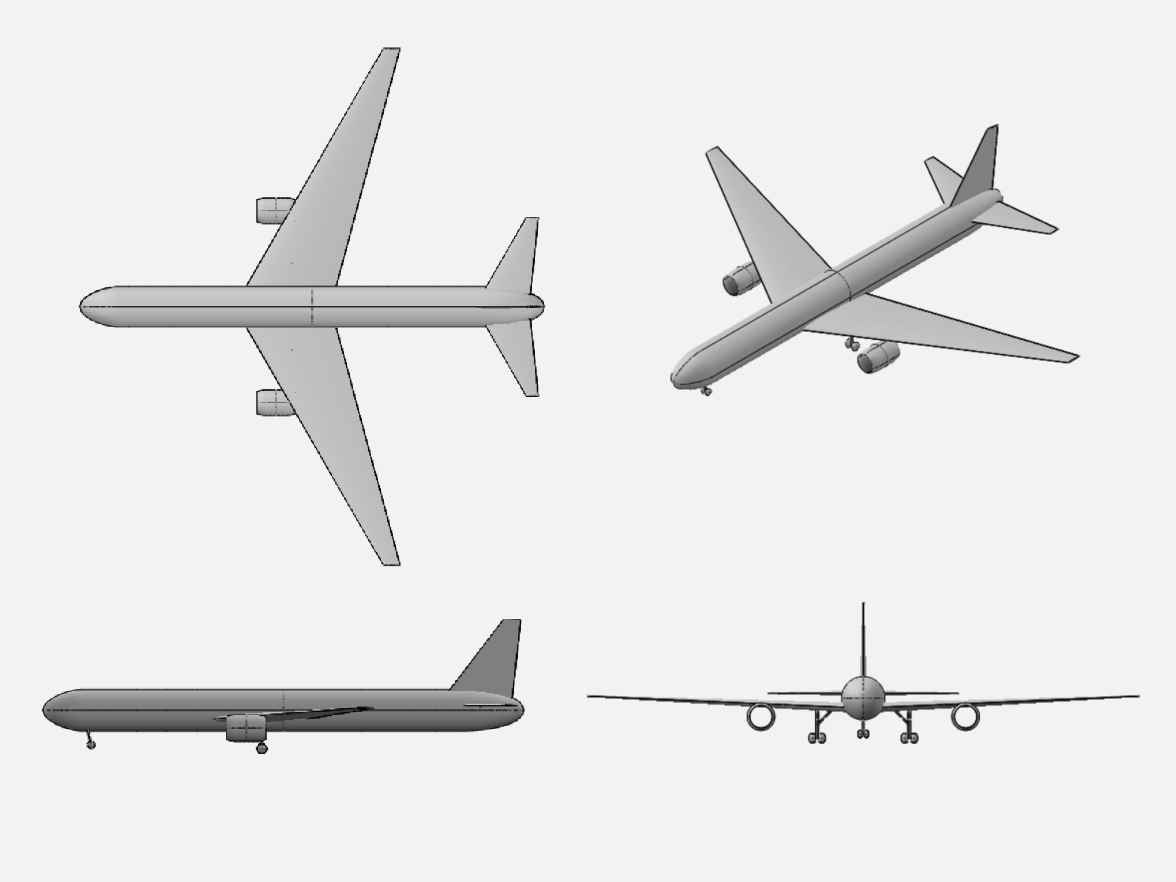
\includegraphics[width=0.6\linewidth]{Photos/3-View_Aircraft_(2-12-20).pdf}
        \caption{3-View Drawing of Sam Mark 1}
        \label{fig3view}
        \end{figure}

\subsection{Internal Configuration}
\subsubsection{Seating Configuration (\textit{JC})}
The aircraft internal configuration is presented as two-class seating combining both business and economy seating accommodations.  Per AIAA RFP \cite{RFP} requirements, the aircraft is designed with 50 business-class and 350 economy-class seats to accommodate 400 total customers.  

\begin{table}[!h]
    \centering
    \caption{Seating Configuration}
    \begin{tabular}{|c|c||c|c|} \toprule
        \multicolumn{2}{c}{\textbf{Business Class}} & \multicolumn{2}{c}{\textbf{Economy Class}} \\ \hline
        Configuration (a) & 2 - 2 - 2 & Configuration (a) & 3 - 4 - 3 \\ \hline
        Row Count (a) & 8 & Row Count (a) & 28 \\ \hline
        Configuration (b) & 1 - 0 - 1 & Configuration (b) & 2 - 3 - 2 \\ \hline
        Row Count (b) & 1 & Row Count (b) & 10 \\ \hline
        Pitch & 36" & Pitch & 32" \\ \hline
        Width & 21" & Width & 18" \\ \bottomrule
    \end{tabular}
    \label{tab:seating}
\end{table}
 
Two different seating configurations are proposed for each class in Table \ref{tab:seating}, above.  The business class contains 8 rows with a 2 - 2 - 2 configuration to provide a spacious flight experience while making efficient use of the space provided.  The purpose of selecting a 2 - 2 - 2 style is to provide business passengers the opportunity to have aisle access.  The 1 - 0 - 1 row is provided to accommodate ADA passengers and may be further customized by the client.  The economy class has two sections with a 3 - 4 - 3 and 2 - 3 - 2 configuration.  The 3 - 4 - 3 section provides high capacity seating while the 2 - 3 - 2 seating enables airliners to offer a highly competitive yet still profitable seating arrangement.

% \subsubsection{Galley Configuration}

% \subsubsection{Lavatory Configuration}

% \subsubsection{Door Configuration}

% \hl{Include Door Certification Requirements} --> are we doing this for DRR?  @NZ



% \textcolor{red}{
% \begin{itemize}
%     \item Discuss external configuration alternatives considered and design choices made.
%     \item Discuss selected aircraft configuration design (i.e. distinctions between variants, major features, design characteristics/objectives).
%     \item Include at least one trade study that uses quantitative or qualitative analysis to support design decisions made.
%     \item Discuss the landing gear philosophy.
%     \item 3-View drawing (VSP acceptable).
%     \item Discuss future work
% \end{itemize}}